\subsection{The standard BD triple}
The initial quiver for $\gc_g^{\dagger}(\bg_{\std},\GL_4)$ is illustrated in Figure~\ref{f:ex_n=4gstd}.

\begin{figure}[htb]
\begin{center}
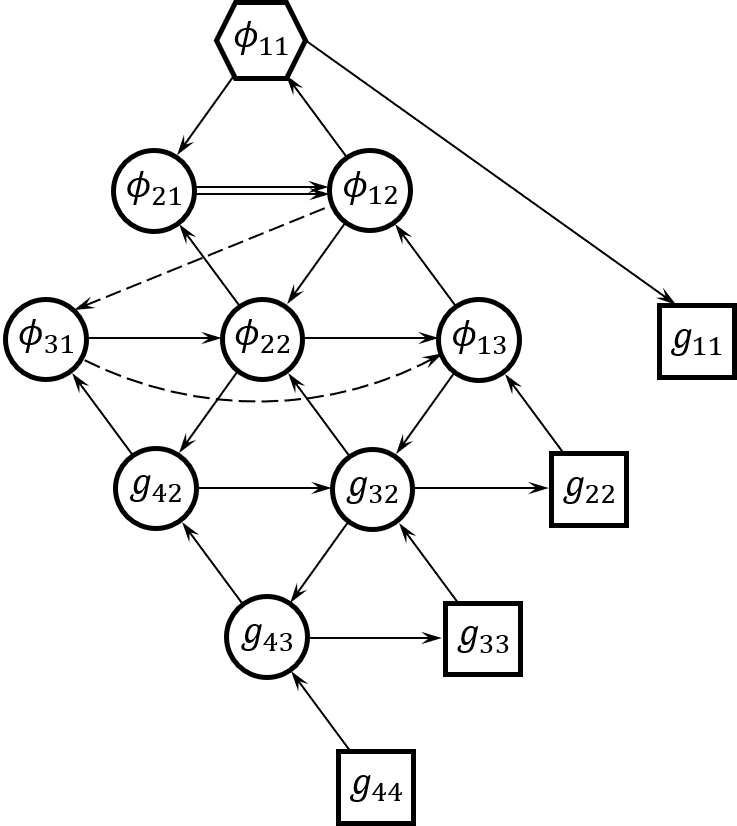
\includegraphics[scale=0.65]{g_convention/g_n=4_std.png}
\end{center}
\caption{The initial quiver for $\gc^{\dagger}_g(\bg_{\std},\GL_4)$.}
\label{f:ex_n=4gstd}
\end{figure}

\paragraph{The initial variables.} The $\phi$- and $c$-variables, as elements of $\mathcal{O}(\GL_4)$, are given by the following formulas:
\begin{align}
    \phi_{11}(U) = \det \begin{bmatrix} u_{21} & (U^2)_{21} & (U^3)_{21} \\ u_{31} & (U^2)_{31} & (U^3)_{31}\\ u_{41} & (U^2)_{41} & (U^3)_{41} \end{bmatrix}, \ \ \phi_{12}(U) = -\det\begin{bmatrix}u_{21} & u_{22} & (U^2)_{21}\\ u_{31} & u_{32} & (U^2)_{31}\\ u_{41} & u_{42} & (U^2)_{41} \end{bmatrix};\\
    \phi_{21}(U) = \det \begin{bmatrix}
        u_{31} & (U^2)_{31} \\ u_{41} & (U^2)_{41}
    \end{bmatrix}, \ \ \phi_{31}(U) = u_{41}, \ \ \phi_{22}(U) = \det U^{[1,2]}_{[3,4]}, \ \ \phi_{13}(U) = \det U^{[1,3]}_{[2,4]};
\end{align}
\begin{align}
    &c_1(U) = -\tr U, \ \ c_2(U) = \frac{1}{2!}\left(\tr(U)^2 - \tr(U^2)\right),\\ &c_3(U) = -\frac{1}{3!}\left( \tr(U)^3 - 3\tr(U)\tr(U^2)+2\tr(U^3)\right).
\end{align}
The $g$-variables are given by
\begin{equation}
    g_{11}(U):=\det U, \ \ g_{ij}(U) = \det U^{[j,n-i+j]}_{[i,n]}, \ \ 2 \leq j \leq i \leq n.
\end{equation}